\documentclass[conference]{IEEEtran}
\usepackage[utf8]{inputenc}
\usepackage[T1]{fontenc}
\usepackage[spanish,es-tabla]{babel}
\usepackage{graphicx}
\usepackage{booktabs}
\usepackage{amsmath}
\usepackage{url}
\usepackage{array}
\usepackage{cite}
\usepackage{float}
\graphicspath{{figuras/}}
\title{Buffer Compartido entre Procesos POSIX: Diseño, Verificación y Evaluación Experimental}
\author{\IEEEauthorblockN{Esteban Chaves Morera, Adrián Campos León y Edwin Loria Fonseca}
\IEEEauthorblockA{Maestría en Ciencias de la Computación\\Tecnológico de Costa Rica\\Sistemas Operativos Avanzados, II semestre de 2026}}
\begin{document}
\maketitle
\begin{abstract}
Se presenta el desarrollo y evaluación de un buffer FIFO compartido entre procesos independientes mediante memoria compartida POSIX. La solución contempla creación, registro de participantes, producción y consumo de mensajes, verificación de integridad y cierre cooperativo. Para su evaluación se emplearon pruebas funcionales y un experimento de 45 corridas, con tres capacidades, tres relaciones entre tasas de producción y consumo y cinco repeticiones por configuración. Los registros permiten comprobar identidad, contenido y conservación de mensajes sin depender del orden físico de escritura de archivos. Los resultados muestran que el incremento de capacidad no implica por sí mismo un mayor rendimiento y que, cuando la producción supera al consumo, puede aumentar considerablemente la latencia de los mensajes. El estudio identifica las garantías del protocolo, contrasta el rendimiento con la latencia y delimita los resultados a las condiciones evaluadas.
\end{abstract}
\begin{IEEEkeywords}
memoria compartida POSIX, sincronización, productor-consumidor, FIFO, concurrencia, experimentación.
\end{IEEEkeywords}

\section{Introducción}
La comunicación entre procesos exige coordinar el acceso a los datos y determinar qué ocurre cuando varios participantes intentan operar al mismo tiempo. En este proyecto se construyó un buffer circular FIFO compartido entre procesos GNU/Linux. Los programas \texttt{creator}, \texttt{producer}, \texttt{consumer} y \texttt{finisher} cumplen funciones diferenciadas. El objetivo no es solamente transferir mensajes: también es conservar su contenido, respetar el orden de extracción y finalizar sin abandonar datos pendientes ni destruir recursos utilizados por otros procesos.

Se presentan la arquitectura del sistema, las reglas de sincronización y cierre, el razonamiento de correctitud, las pruebas y el análisis experimental. El estudio utiliza los resultados registrados por el equipo y distingue las propiedades del protocolo de las observaciones obtenidas en las corridas.

\section{Arquitectura y protocolo de sincronización}

\subsection{Disposición de la memoria compartida}
Cada instancia corresponde a un objeto de memoria compartida POSIX identificado por el valor validado de \texttt{--name}. El creador obtiene el objeto mediante \texttt{shm\_open}, calcula su tamaño, lo dimensiona y lo proyecta con \texttt{mmap}. Los demás ejecutables abren el mismo nombre y realizan su propio mapeo; por ello, una instancia puede aparecer en direcciones virtuales diferentes en cada proceso. La representación compartida no almacena punteros: utiliza índices, identificadores y tipos enteros de ancho fijo.

El segmento está compuesto por una cabecera de tamaño fijo seguida por un arreglo flexible de mensajes. Su tamaño se calcula como
\begin{equation}
S=\operatorname{offsetof}(\textit{SharedInstance},\textit{messages})
  + C\,\operatorname{sizeof}(\textit{Message}),
\end{equation}
donde $C$ es la capacidad solicitada, limitada al intervalo de 1 a 1024 mensajes. Antes de utilizar cualquier primitiva de sincronización, el proceso que se conecta contrasta el tamaño obtenido mediante \texttt{fstat} con el tamaño declarado en la cabecera y valida el número mágico, la versión de la ABI y la capacidad.

\begin{table}[htbp]
\caption{Organización de la instancia compartida}\label{tab:memoria}
\centering\footnotesize
\begin{tabular}{p{.29\columnwidth}p{.61\columnwidth}}
\toprule
Componente & Propósito \\
\midrule
Identificación & Número mágico, versión de ABI, tamaño del mapeo, capacidad y estado de publicación \\
Sincronización & Mutex y condiciones para espacio, datos y cambios de estado \\
Ciclo de vida & Estado operativo y marca que reserva el único finalizador \\
Buffer circular & Índices de entrada y salida, ocupación y arreglo flexible de mensajes \\
Participantes & Contadores activos y mapas de bits de identificadores usados por cada rol \\
Métricas & Secuencias, cantidades aceptadas y extraídas, tiempos globales y acumuladores por participante \\
\bottomrule
\end{tabular}
\end{table}

El mensaje almacenado tiene tamaño fijo y contiene el identificador del productor, su secuencia local, la secuencia global de inserción, la marca monotónica de aceptación y una carga útil de 32 bytes. La carga no contiene texto, direcciones ni referencias a memoria privada. Puede reconstruirse a partir de la identidad lógica del mensaje, lo que permite detectar alteraciones después de la extracción. El cierre tampoco se codifica como un mensaje especial: se comunica mediante el estado de la instancia y las variables de condición, de modo que los contadores representen únicamente mensajes de datos.

La arquitectura diferencia el estado de publicación del estado operativo. La publicación evoluciona entre \texttt{INITIALIZING}, \texttt{READY} y \texttt{RETIRED}, y evita que un proceso utilice una representación incompleta o primitivas ya destruidas. Por separado, el estado operativo controla las transiciones \texttt{OPEN}, \texttt{CLOSING} y \texttt{CLOSED}. Esta separación permite resolver tanto las operaciones normales del buffer como las carreras entre creación, conexión y destrucción.

Existen dos niveles de protección con un orden fijo. Primero se adquiere sobre el descriptor un bloqueo de registro \texttt{fcntl}, de lectura para procesos conectados o de escritura para creación y destrucción; después, cuando corresponde, se adquiere el mutex ubicado en memoria compartida. Nunca se solicita el bloqueo del descriptor mientras se posee el mutex. Cada participante conserva el bloqueo de lectura desde antes de mapear hasta después de dejar de utilizar las primitivas, impidiendo que el finalizador las destruya mientras permanece una conexión activa.

El mutex y las variables de condición se inicializan con el atributo \texttt{PTHREAD\_PROCESS\_SHARED}. El mutex protege conjuntamente el estado operativo, los índices, la ocupación, los registros de participantes, las secuencias y los acumuladores. Las condiciones \texttt{not\_full}, \texttt{not\_empty} y \texttt{state\_changed} separan las esperas por espacio, por datos y por cambios relevantes para el cierre. La elección de un único mutex simplifica los invariantes y evita órdenes de adquisición internos incompatibles, a cambio de serializar las modificaciones del estado compartido.

Cada proceso mantiene además un descriptor privado, la dirección y longitud de su mapeo, su rol, identificador y condición de registro. El generador pseudoaleatorio, el escritor CSV y cualquier memoria obtenida dinámicamente también son privados. No se comparten objetos \texttt{FILE}, rutas, estados del generador ni direcciones virtuales. Cuando termina, cada proceso libera solamente su mapeo y descriptor; el único finalizador es responsable de destruir las primitivas y retirar el nombre de memoria compartida después de comprobar que ya no existen usuarios.

\subsection{Pseudocódigo de las operaciones}
El siguiente pseudocódigo resume las operaciones que modifican el estado compartido. Se denota por $M$ el mutex de la instancia. Cada proceso que alcanza estas funciones ya conserva el bloqueo de lectura sobre el descriptor, por lo que el mapeo y las primitivas permanecen válidos. Los eventos se capturan dentro de la sección crítica, pero su escritura en CSV ocurre después de liberar $M$.

El registro comprueba conjuntamente el estado y la unicidad del identificador. El mapa de bits no se limpia durante la retirada, de modo que un identificador no pueda reutilizarse dentro de la misma instancia.

{\footnotesize
\begin{verbatim}
registrar(rol, id):
  lock(M)
  si estado != OPEN:
    unlock(M); retornar CERRADO
  si id no valido:
    unlock(M); retornar ID_INVALIDO
  si usado[rol][id]:
    unlock(M); retornar DUPLICADO
  usado[rol][id] <- verdadero
  activos[rol] <- activos[rol] + 1
  marcar metricas[id] como activas
  capturar evento JOIN
  broadcast(state_changed)
  unlock(M)

retirar(rol, id):
  lock(M)
  activos[rol] <- activos[rol] - 1
  marcar metricas[id] como inactivas
  capturar evento LEAVE
  broadcast(state_changed)
  unlock(M)
\end{verbatim}
}

Antes de confirmar su retirada, cada trabajador vacía los eventos de datos de su archivo CSV. El consumidor completa además el procesamiento del mensaje que haya extraído. Durante el desregistro se captura el evento \texttt{LEAVE} en memoria privada y se marca al participante como inactivo, conservando sus acumuladores compartidos. El trabajador escribe ese último evento y cierra el archivo antes de liberar su conexión, por lo que la destrucción de recursos no puede adelantarse a esas operaciones.

En la inserción, la espera se mantiene únicamente mientras la instancia continúa abierta y el buffer está lleno. La asignación de tiempo y secuencia global ocurre en la misma región crítica que el cambio de estado; el incremento de mensajes aceptados es el punto de efecto de la operación.

{\footnotesize
\begin{verbatim}
insertar(borrador):
  lock(M)
  mientras estado = OPEN y ocupacion = capacidad:
    wait(not_full, M)
  si estado != OPEN:
    unlock(M); retornar CERRADO
  comprobar desbordamientos
  mensaje <- borrador
  mensaje.enqueue_seq <- siguiente_insercion++
  mensaje.tiempo <- reloj_monotonico()
  mensajes[tail] <- mensaje
  tail <- (tail + 1) mod capacidad
  ocupacion <- ocupacion + 1
  aceptados <- aceptados + 1
  capturar evento ENQUEUE
  signal(not_empty)
  unlock(M)
\end{verbatim}
}

La extracción usa el predicado complementario. Un consumidor espera solamente cuando el buffer está vacío y la instancia sigue abierta. Durante \texttt{CLOSING} puede continuar mientras haya mensajes; cuando observa cierre y ocupación cero termina sin extraer. La disminución de la ocupación y el incremento de extraídos forman su punto de efecto.

{\footnotesize
\begin{verbatim}
extraer():
  lock(M)
  mientras ocupacion = 0 y estado = OPEN:
    wait(not_empty, M)
  si ocupacion = 0:
    unlock(M); retornar CERRADO
  comprobar desbordamientos
  mensaje <- mensajes[head]
  head <- (head + 1) mod capacidad
  ocupacion <- ocupacion - 1
  extraidos <- extraidos + 1
  asignar dequeue_seq y tiempo de extraccion
  capturar evento DEQUEUE
  signal(not_full)
  si ocupacion = 0: broadcast(state_changed)
  unlock(M)
  procesar mensaje y escribir CSV fuera de M
\end{verbatim}
}

El productor realiza su pausa antes de intentar insertar y calcula una sola vez un plazo absoluto con reloj monotónico. La espera temporizada sobre \texttt{state\_changed} libera el mutex mientras el proceso permanece bloqueado. Cuando recibe una notificación vuelve a comprobar el estado y el plazo original, sin reiniciar la demora sorteada. Si comienza el cierre, abandona la pausa y se retira sin insertar. El consumidor procesa después de extraer y permanece registrado hasta completar ese trabajo privado, incluso si el cierre ya fue solicitado.

El finalizador primero reclama de forma exclusiva la conducción del cierre. Si existen productores activos o mensajes pendientes sin consumidores, revierte esa reclamación y deja la instancia en \texttt{OPEN}. En otro caso establece el punto de corte, despierta a todos los participantes y espera sobre una condición, sin sondeo periódico.

{\footnotesize
\begin{verbatim}
finalizar():
  lock(M)
  si estado != OPEN:
    unlock(M); retornar CERRADO
  si finalizador_reclamado:
    unlock(M); retornar OCUPADO
  finalizador_reclamado <- verdadero
  si consumidores = 0 y
     (productores > 0 o ocupacion > 0):
    finalizador_reclamado <- falso
    unlock(M); retornar SIN_CONSUMIDOR
  estado <- CLOSING
  guardar tiempo de corte
  broadcast(not_full, not_empty, state_changed)
  mientras ocupacion > 0 o productores > 0 o
           consumidores > 0:
    wait(state_changed, M)
  estado <- CLOSED
  copiar resumen a memoria privada
  unlock(M)

  liberar bloqueo de lectura del descriptor
  adquirir bloqueo de escritura del descriptor
  // espera aqui conexiones aun no registradas
  publicacion <- RETIRED
  destruir condiciones y mutex
  shm_unlink(nombre); munmap; close
  retornar resumen privado
\end{verbatim}
}

Las comprobaciones se ejecutan dentro de ciclos porque POSIX permite despertares espurios y porque otro proceso puede modificar el predicado antes de que quien despertó recupere el mutex. De esta forma, una notificación solo indica que conviene volver a evaluar el estado; no garantiza por sí misma que la operación pueda avanzar.

\subsection{Modelo de estados y protocolo de cierre}
El ciclo de vida de una instancia se representa mediante los estados \texttt{OPEN}, \texttt{CLOSING} y \texttt{CLOSED}. En \texttt{OPEN} se permite registrar participantes y aceptar mensajes de los productores. Los consumidores pueden extraer mensajes disponibles o esperar de forma bloqueante cuando el buffer está vacío. De manera análoga, un productor espera espacio cuando el buffer está lleno. Estas esperas se realizan sobre predicados protegidos por el mutex y se comprueban nuevamente después de cada despertar.

La transición de \texttt{OPEN} a \texttt{CLOSING} constituye el punto de corte del cierre. El finalizador la realiza bajo la misma exclusión mutua utilizada para aceptar mensajes, de modo que cada inserción queda ordenada antes o después del corte. Una vez iniciada esta transición no se admiten nuevos participantes ni nuevas inserciones. Los productores bloqueados o en pausa deben despertar, observar el cambio de estado y retirarse sin insertar otro mensaje. Los consumidores, en cambio, continúan extrayendo hasta vaciar el buffer y completan fuera de la región crítica el procesamiento privado de los mensajes ya obtenidos.

El cierre cooperativo sigue la siguiente secuencia:
\begin{enumerate}
\item El finalizador comprueba que el cierre puede progresar sin dejar mensajes sin consumidor y que no existe otro finalizador conduciendo el protocolo.
\item Bajo el mutex, cambia el estado a \texttt{CLOSING} y notifica a productores y consumidores que podrían encontrarse esperando.
\item Los productores dejan de generar inserciones y confirman su retirada; los consumidores drenan los mensajes pendientes antes de retirarse.
\item El finalizador espera sobre \texttt{state\_changed} hasta que el buffer esté vacío y no queden participantes activos.
\item Al retirarse los participantes, la instancia pasa a \texttt{CLOSED}. El finalizador libera su bloqueo de lectura y espera después el bloqueo exclusivo del descriptor; esta segunda espera cubre conexiones abiertas que nunca llegaron a registrarse. Solamente entonces destruye los recursos y permite reutilizar el nombre.
\end{enumerate}

La retirada de un participante no equivale al cierre global. Un buffer temporalmente vacío tampoco implica que la ejecución haya terminado, porque aún pueden existir productores activos o consumidores procesando mensajes previamente extraídos. Por ello, las decisiones de avance dependen conjuntamente del estado, la ocupación, los participantes registrados y las conexiones en curso. Este criterio evita destruir las primitivas compartidas mientras otro proceso todavía puede acceder a ellas.

\subsection{Correctitud, progreso y ausencia de interbloqueo}
El razonamiento de correctitud parte de que todas las modificaciones del buffer y del estado operativo se realizan bajo el mismo mutex. Si $O$ representa la ocupación y $C$ la capacidad, el invariante principal es
\begin{equation}
0 \leq O \leq C.
\end{equation}
Inicialmente $O=0$. Una inserción solo incrementa la ocupación después de comprobar $O<C$, y una extracción solo la disminuye cuando $O>0$. Como ambas operaciones son mutuamente excluyentes, una inducción sobre la secuencia de operaciones conserva el límite para cualquier intercalado permitido.

La conservación de mensajes se expresa como
\begin{equation}
A=E+O,
\end{equation}
donde $A$ es la cantidad aceptada y $E$ la cantidad extraída. Una inserción válida incrementa simultáneamente $A$ y $O$; una extracción incrementa $E$ y disminuye $O$. Ninguna operación posterior al punto de corte puede incrementar $A$. Al alcanzar \texttt{CLOSED}, el predicado de drenaje exige $O=0$, por lo que $A=E$ durante un cierre normal.

La propiedad FIFO se obtiene de los índices \texttt{tail} y \texttt{head}. Cada productor escribe exclusivamente en la posición señalada por \texttt{tail} y después lo avanza de forma circular; cada consumidor lee exclusivamente desde \texttt{head} y lo avanza de la misma forma. La secuencia global \texttt{enqueue\_seq} identifica el orden de aceptación y \texttt{dequeue\_seq} el de extracción. Como una celda no puede extraerse antes de ser aceptada ni reutilizarse mientras forma parte de la ocupación, el orden de extracción coincide con el orden de aceptación. El procesamiento privado puede finalizar en otro orden sin violar el FIFO del buffer.

Los puntos de efecto permiten clasificar operaciones concurrentes como si hubieran ocurrido atómicamente. El registro tiene efecto cuando se marca el identificador y aumenta el contador activo; la inserción, cuando se publica el mensaje y aumenta la ocupación; la extracción, cuando disminuye la ocupación y se contabiliza el mensaje; y el cierre, cuando el estado cambia a \texttt{CLOSING}. En particular, una inserción concurrente con el cierre queda completamente antes del corte o es rechazada después de él, porque ambas decisiones se toman bajo el mismo mutex.

No se forma un ciclo de espera entre los participantes durante una ejecución cooperante. Solo existe un mutex compartido y \texttt{pthread\_cond\_wait} lo libera mientras el proceso duerme. Un productor que inserta señala \texttt{not\_empty}; un consumidor que extrae señala \texttt{not\_full}; y el finalizador difunde las tres condiciones al cambiar el estado. Además, el finalizador libera el mutex antes de abandonar su bloqueo de lectura y solicitar el bloqueo de escritura del descriptor. De esta forma se respeta siempre el orden descriptor--mutex y no aparece una adquisición circular entre ambos niveles.

El argumento de progreso supone procesos cooperantes y una planificación que permita ejecutar eventualmente a algún participante habilitado. Si hay mensajes y un consumidor activo, este puede extraer; si hay espacio y un productor activo, este puede insertar; y durante el cierre los consumidores pueden drenar mientras los productores dejan de generar trabajo. Sin embargo, POSIX no garantiza equidad entre quienes esperan un mutex o una condición. Por ello, el protocolo no promete espera temporalmente acotada ni ausencia absoluta de inanición para un participante particular, aunque las pruebas ejecutadas sí comprueban progreso en los escenarios descritos.

La seguridad del ciclo de vida se apoya en los bloqueos incompatibles del descriptor. Toda conexión capaz de utilizar una primitiva conserva un bloqueo de lectura, mientras que la destrucción requiere el bloqueo de escritura. En consecuencia, el finalizador no puede destruir el mutex o las condiciones mientras exista un proceso con derecho a utilizarlos. Este razonamiento cubre el cierre cooperativo, pero no pretende recuperar una instancia si un proceso termina abruptamente dentro de una región crítica ni sustituye el análisis dinámico con sanitizadores.

\subsection{Análisis de complejidad y escalabilidad}
La inserción y la extracción en el buffer circular tienen complejidad temporal constante, $O(1)$. Cada operación accede a una posición determinada por los índices de entrada o salida, actualiza la ocupación y avanza el índice correspondiente mediante aritmética circular. No es necesario desplazar mensajes ni recorrer el buffer. Estas actualizaciones se realizan dentro de una sección crítica para conservar la relación entre índices, ocupación y secuencias globales.

El espacio requerido por la estructura compartida es $O(C)$, donde $C$ representa la capacidad configurada. La cabecera, los índices, el estado y los contadores ocupan espacio constante, mientras que el arreglo de mensajes crece linealmente con la capacidad. A esto se suman las estructuras de control de participantes y los datos privados de cada proceso, como su generador de pausas y archivo CSV. Aumentar la capacidad incrementa la memoria disponible para mensajes pendientes, pero no añade capacidad de procesamiento a los consumidores.

La complejidad constante de las operaciones no implica que el rendimiento aumente linealmente con la cantidad de procesos. Todos los productores y consumidores compiten por el mismo mutex para modificar el estado compartido, por lo que la actualización efectiva del buffer se serializa. Conforme crece la concurrencia también pueden aumentar la contención, los cambios de contexto y el costo de despertar procesos. El uso de variables de condición evita consumir CPU mediante espera activa, aunque cada despertar todavía requiere volver a adquirir el mutex y comprobar el predicado correspondiente.

El trabajo privado, incluidas las pausas, el procesamiento simulado y la escritura de los CSV, se mantiene fuera de la región crítica. Esta separación reduce el tiempo durante el cual se bloquea a otros participantes, pero no elimina el costo global de planificación y entrada/salida. En particular, los registros pueden afectar las mediciones aun cuando no se escriban bajo el mutex, debido a la actividad adicional del sistema de archivos.

Los resultados experimentales concuerdan con estas limitaciones. Cuando la producción fue más rápida que el consumo, ampliar la capacidad de 1 a 64 mensajes no produjo un aumento apreciable del rendimiento, pero elevó considerablemente la latencia. Una capacidad mayor absorbe ráfagas y permite que los productores avancen durante más tiempo; sin embargo, si la tasa de consumo constituye el límite, los mensajes adicionales solamente permanecen acumulados. Por tanto, la capacidad debe seleccionarse como un compromiso entre tolerancia a ráfagas, uso de memoria y tiempo de espera, y no como un mecanismo que garantice mayor escalabilidad.


\subsection{Fundamentación y decisiones de diseño}

\subsubsection{Buffer acotado de Dijkstra}
Las secciones 3.2 y 3.3 de \textit{Cooperating Sequential Processes} presentan primitivas de sincronización y su aplicación a la exclusión mutua; las secciones 4.1 y 4.3 desarrollan usos del semáforo general y el buffer acotado, respectivamente \cite{dijkstra}. La distinción central es que la exclusión protege la modificación de una representación compartida, mientras que los permisos expresan cuántas operaciones pueden avanzar. En una formulación clásica se emplea un contador de espacios libres, otro de elementos disponibles y una exclusión para modificar la cola.

El orden de esas operaciones es parte del algoritmo. Un productor debe reservar un espacio antes de entrar a modificar el buffer y publicar un elemento disponible solamente después de completar la inserción. El consumidor realiza el proceso complementario: reserva un elemento, lo extrae bajo exclusión y después publica un espacio libre. Si se invierten pasos o se espera un permiso mientras se conserva la exclusión que necesita la contraparte, puede exponerse un elemento incompleto o impedirse el progreso.

Durante una operación en curso no es correcto suponer que la suma instantánea de los contadores de elementos y espacios libres coincide siempre con la capacidad. Por ejemplo, un productor puede haber decrementado el semáforo de espacios y estar esperando la exclusión antes de publicar el elemento; ese permiso está reservado, pero todavía no aparece como dato disponible. La conservación debe razonarse incluyendo esas operaciones en tránsito, no únicamente observando los valores momentáneos de los semáforos.

La implementación adopta los mismos principios con una representación diferente. La variable \texttt{occupancy}, leída y escrita únicamente bajo el mutex, determina los predicados $O<C$ para productores y $O>0$ para consumidores. Las condiciones \texttt{not\_full} y \texttt{not\_empty} no representan permisos acumulados: notifican que el predicado puede haber cambiado. Así, capacidad, exclusión y orden de publicación permanecen explícitos en un único estado protegido.

\subsubsection{Mutex y condiciones según Birrell}
Birrell separa el acceso exclusivo a datos compartidos de la planificación de quienes esperan utilizarlos. La sección \textit{Using a Mutex: accessing shared data} asocia cada conjunto de datos con un mutex y exige acceder a ellos bajo esa protección. La sección \textit{Using a Condition variable: scheduling shared resources} explica que una condición se vincula con el mutex y con un predicado sobre los datos protegidos; \textit{Wait} libera atómicamente el mutex, bloquea al participante y lo readquiere antes de retornar \cite{birrell}.

Esta separación aparece directamente en el prototipo. El mutex conserva los invariantes de ocupación, índices, participantes y estado. Las variables de condición coordinan esperas diferentes, pero ninguna sustituye la comprobación de los datos: al despertar, el proceso vuelve a evaluar el predicado dentro de un ciclo. Una señal no transfiere la propiedad de un mensaje o espacio, y puede no tener efecto si nadie espera; la corrección depende del estado protegido, no de recordar notificaciones.

Birrell describe hilos que comparten naturalmente un espacio de direcciones. En este proyecto los participantes son procesos independientes, por lo que la aplicación de esas ideas requiere diferencias concretas: los datos se colocan en un objeto \texttt{mmap}, no se almacenan punteros privados y las primitivas se configuran con \texttt{PTHREAD\_PROCESS\_SHARED}. Además, debe protegerse la vida del mapeo para que ningún proceso destruya una condición o mutex que otro todavía pueda utilizar. El bloqueo de descriptor y los estados de publicación atienden este problema adicional, que no se resuelve únicamente con el monitor descrito para hilos.

\subsubsection{Comparación conceptual con semáforos}
Una alternativa POSIX podría emplear semáforos contadores para elementos y espacios, además de un semáforo binario o mutex para la estructura circular. Esta representación hace explícitos los permisos descritos por Dijkstra y resulta natural durante la operación estable. No obstante, el cierre exigiría un mecanismo adicional para distinguir permisos reales de despertares destinados a terminar, impedir nuevas reservas y liberar a todos los procesos bloqueados sin fabricar mensajes o espacios inexistentes.

El esquema elegido concentra la verdad del protocolo en el estado protegido: ocupación, capacidad y estado operativo. El cierre cambia a \texttt{CLOSING} y realiza difusiones; cada participante despierta y decide con el predicado si debe avanzar o terminar. Como contraparte, todos deben seguir rigurosamente el patrón de ciclo, espera y nueva comprobación, y la adquisición del único mutex puede convertirse en un punto de contención. La comparación no implica una segunda implementación: ambas alternativas pueden ser correctas si mantienen el orden de operaciones, pero mutex y condiciones se ajustan mejor al predicado de cierre compuesto utilizado por este prototipo.

\subsubsection{Decisiones concretas del prototipo}
\textbf{Granularidad del bloqueo.} Se utiliza un único mutex para proteger estado, buffer, participantes, secuencias y acumuladores. Dividirlo en varios bloqueos podría permitir que algunas operaciones avanzaran en paralelo, pero obligaría a establecer un orden de adquisición y haría más difícil obtener instantáneas coherentes durante el cierre. La granularidad elegida simplifica los invariantes y permite ordenar con claridad una inserción frente al punto de corte. Su costo es que incluso operaciones sobre datos conceptualmente distintos compiten por la misma exclusión; por ello, la sección crítica se limita a las actualizaciones indispensables.

\textbf{Capacidad fija y buffer circular.} La capacidad se decide al crear la instancia y no cambia durante su vida. Esto permite calcular una única proyección de memoria, representar las posiciones mediante índices y ejecutar inserción y extracción en $O(1)$. Un redimensionamiento exigiría coordinar nuevos mapeos en procesos independientes y actualizar la representación sin dejar direcciones o tamaños incompatibles. La capacidad fija evita ese riesgo, aunque obliga a elegir de antemano el compromiso entre memoria, absorción de ráfagas y latencia. Los resultados confirman que una capacidad mayor no garantiza más rendimiento y puede prolongar la permanencia de mensajes en cola.

\textbf{Captura protegida y escritura diferida de registros.} Los campos que describen una operación se copian a un evento privado mientras se posee el mutex; el CSV se escribe después de liberarlo. Escribir dentro de la región crítica produciría un orden físico más directo, pero convertiría la latencia del sistema de archivos en tiempo de bloqueo para todos los participantes. La decisión adoptada reduce la contención y conserva una secuencia lógica verificable. Como consecuencia, el orden de las líneas entre archivos no representa el orden de ejecución y un error de escritura no puede revertir un mensaje que ya fue aceptado o extraído.

\textbf{Identificadores históricos sin memoria dinámica compartida.} Los identificadores válidos se conservan en mapas de bits separados por rol y no se liberan cuando un participante se retira. Las métricas se almacenan en arreglos indexados por esos identificadores. Esta decisión permite comprobar duplicados en tiempo constante y evita punteros o asignadores dentro del segmento compartido. El costo es reservar espacio para el límite máximo y prohibir la reutilización de un identificador durante la misma instancia, incluso si su participante ya terminó.

\textbf{Cierre explícito y protección del ciclo de vida.} El protocolo combina estados operativos, una reclamación de finalizador y bloqueos de descriptor. Una solución más simple podría eliminar el nombre al cambiar a \texttt{CLOSING}, pero no impediría que un proceso que ya abrió el objeto intentara utilizar primitivas durante su destrucción. Mantener un bloqueo de lectura por conexión y exigir uno de escritura para destruir añade pasos al cierre, pero establece una frontera comprobable: mientras exista un usuario potencial, la destrucción no puede avanzar. Esta complejidad se acepta para permitir cierre cooperativo, conexiones concurrentes y reutilización segura del nombre.

Estas decisiones priorizan una representación verificable y un razonamiento de cierre claro sobre el máximo paralelismo posible. La evaluación experimental permite observar el costo conjunto, pero no atribuir toda variación a una sola decisión; por ejemplo, la contención del mutex, la planificación y la escritura diferida de registros pueden coincidir en una misma corrida.

\section{Métricas y verificación de mensajes}
\subsection{Registro y correspondencia de eventos}
Cada participante escribe un archivo CSV de eventos con versión, rol, identificador, evento, tiempo monotónico, estado y datos del mensaje. La identidad lógica de cada mensaje está definida por el par \((\textit{producer\_id},\textit{sequence})\). Los mensajes insertados y extraídos se cruzan mediante esta identidad, mientras que los campos \texttt{enqueue\_seq} y \texttt{dequeue\_seq} permiten reconstruir el orden global de las operaciones.

Este diseño evita un error frecuente: asumir que la primera línea escrita en un archivo ocurrió antes que una línea de otro archivo. En este sistema, el evento se obtiene dentro de la sección crítica y la escritura CSV se realiza fuera del mutex; por eso, el orden físico de escritura no constituye evidencia suficiente para afirmar FIFO. El verificador también comprueba la carga útil reproducible, las secuencias faltantes o repetidas y la conservación de los datos al finalizar.

\subsection{Medidas obtenidas}
El resumen de cierre registra mensajes aceptados, extraídos y pendientes, marcas de inicio y liberación, rendimiento y duración. La conservación se comprueba con la relación:
\begin{equation}
N_{\mathrm{aceptados}}=N_{\mathrm{extraidos}}+N_{\mathrm{pendientes}}.
\end{equation}
Al concluir normalmente, el valor esperado es \(N_{\mathrm{pendientes}}=0\). El rendimiento se expresa en mensajes por segundo, a partir de la cantidad extraída y del intervalo operativo informado por el resumen. La latencia de cada mensaje corresponde al tiempo transcurrido entre su aceptación y su extracción, no al procesamiento privado posterior. El percentil 95 complementa el promedio al describir las observaciones de mayor espera.

El verificador compara los eventos \texttt{JOIN} y \texttt{ENQUEUE} con el instante de transición a \texttt{CLOSING}. La salida \texttt{LEAVE} puede ocurrir durante el cierre, al igual que las extracciones necesarias para drenar el buffer. Las marcas permiten auditar los registros, mientras que la exclusión entre insertar y cambiar de estado depende de la sincronización implementada en C.

\section{Pruebas de funcionamiento e integridad}
La suite automatizada puede ejecutarse mediante \texttt{make -j4 test}; el comando finaliza con código distinto de cero cuando falla una condición comprobada. Se realizaron pruebas de argumentos, funcionamiento FIFO, concurrencia, capacidades mínimas, bloqueo y reanudación, así como cierre y corrupción de registros.

\begin{table*}[htbp]
\caption{Evidencia seleccionada de pruebas funcionales}\label{tab:pruebas}
\centering\footnotesize
\setlength{\tabcolsep}{3pt}
\begin{tabular}{p{.09\textwidth}p{.17\textwidth}p{.25\textwidth}p{.31\textwidth}p{.09\textwidth}}
\toprule
Caso & Comando & Resultado esperado & Resultado obtenido & Conclusión \\
\midrule
T01 & \texttt{make test-options} & Rechazo de argumentos inválidos sin alterar instancias & 264 casos del analizador aprobados & Aprobado \\
T02--T04 & \texttt{make test-buffer} & FIFO y conservación con 1000/4000 mensajes y capacidades 8/1 & Conteos completos, cargas íntegras y secuencias FIFO verificadas & Aprobado \\
T05--T06 & \texttt{make test-workers} & Bloqueo y reanudación con buffer lleno o vacío & Los procesos esperaron y reanudaron sin sondeo & Aprobado \\
T07--T11 & \texttt{make test-shutdown} & Corte, drenaje, retirada, exclusión de finalizadores y reutilización & Intercalados aprobados; 50 repeticiones consecutivas sin fallo & Aprobado \\
T12 & \texttt{make test-stress} & 32 productores/32 consumidores, sin pérdidas ni bloqueo permanente & 32\,000 mensajes verificados en capacidades 1 y 8 & Aprobado \\
T13 & \texttt{make test-sanitizers} & Suite sin accesos inválidos ni comportamiento indefinido & ASan y UBSan aprobaron; LeakSanitizer se deshabilitó bajo \texttt{ptrace} & Aprobado con límite \\
P2-11 & \texttt{verificar\_csv.py} & Rechazar corrupción y operaciones posteriores al corte & Diagnóstico correcto y código distinto de cero & Aprobado \\
\bottomrule
\end{tabular}
\end{table*}

La suite integrada ejecutó 71 pruebas Python, 264 casos del analizador de argumentos y las suites C, con código final cero. Además, se verificó una corrida real con 800 mensajes aceptados y 800 extraídos. Al alterar deliberadamente la duración de cierre del resumen, el verificador informó el campo incorrecto y devolvió código 1; igualmente rechazó una inserción simulada posterior al corte. En P2-13 se documentaron 50 repeticiones consecutivas de pruebas de cierre. Estas evidencias corresponden a ejecuciones observadas y no constituyen una demostración formal de ausencia de todas las carreras posibles.

\subsection{Estrés y análisis dinámico}
El caso de estrés ejecuta 32 productores y 32 consumidores independientes, pausas desactivadas y 1000 mensajes por productor. Para capacidades 1 y 8 se verificaron 32\,000 mensajes, FIFO, integridad, cierre y eliminación del nombre POSIX. La misma suite se reconstruyó con AddressSanitizer y UndefinedBehaviorSanitizer. ASan no detectó accesos inválidos con \texttt{detect\_leaks=0}; la detección de fugas se deshabilitó porque LeakSanitizer no funciona bajo \texttt{ptrace} en el entorno WSL2 utilizado. UBSan no informó comportamiento indefinido. Los sanitizadores complementan las pruebas e invariantes, pero no detectan por sí mismos carreras entre procesos ni demuestran progreso para todo intercalado.

\section{Trazabilidad de requisitos}
La Tabla~\ref{tab:trazabilidad} relaciona los requisitos principales con el mecanismo utilizado para atenderlos y con la evidencia mencionada en este informe. Esta correspondencia permite distinguir entre propiedades respaldadas por pruebas ejecutadas y actividades que todavía deben completarse antes de la entrega definitiva.

\begin{table*}[htbp]
\caption{Correspondencia entre requisitos, mecanismos y evidencia}\label{tab:trazabilidad}
\centering\footnotesize
\begin{tabular}{p{.19\textwidth}p{.35\textwidth}p{.37\textwidth}}
\toprule
Requisito & Mecanismo de cumplimiento & Evidencia o estado \\
\midrule
Comunicación entre procesos independientes & Segmento de memoria compartida POSIX y estructuras sin punteros privados; conexión por nombre de instancia & Construcción y ejecución de \texttt{creator}, \texttt{producer}, \texttt{consumer} y \texttt{finisher} \\
Exclusión mutua y espera bloqueante & Mutex y variables de condición compartidos entre procesos; predicados comprobados después de cada despertar & T05--T06 comprueban bloqueo y reanudación con buffer lleno o vacío \\
Orden FIFO & Índices circulares y secuencias globales \texttt{enqueue\_seq} y \texttt{dequeue\_seq} & T02 y T03 verifican 1000 y 4000 mensajes, respectivamente; T04 cubre capacidad 1 \\
Ausencia de pérdidas, duplicaciones y alteraciones & Identidad $(\textit{producer\_id},\textit{sequence})$, carga reproducible y cruce automatizado de eventos & Corrida real con 800 mensajes aceptados y extraídos; trazas alteradas son rechazadas por P2-11 \\
Cierre cooperativo y drenaje & Estados \texttt{OPEN}, \texttt{CLOSING} y \texttt{CLOSED}; corte de inserciones y retirada coordinada & P2-13 registra 50 repeticiones de escenarios de cierre; P2-11 rechaza inserciones posteriores al corte \\
Medición reproducible & CSV por participante, reloj monotónico, resumen final y fórmulas documentadas & Verificador automatizado y datos agregados provenientes de archivos publicados en \texttt{results/experimentos} \\
Evaluación de capacidad y tasas & Matriz de tres capacidades, tres relaciones de tasas y cinco repeticiones & 45 corridas verificadas, 36\,000 mensajes y resultados de la Tabla~\ref{tab:resultados} \\
Detección de errores de memoria y comportamiento indefinido & Compilación y ejecución con AddressSanitizer y UndefinedBehaviorSanitizer & Suite y estrés aprobados; limitación de LeakSanitizer documentada en P2-14 \\
Reconstrucción y ejecución automatizada & Objetivos \texttt{make clean}, \texttt{make -j4} y \texttt{make -j4 test} & Reconstrucción local limpia aprobada; P2-17 repetirá desde una copia independiente \\
\bottomrule
\end{tabular}
\end{table*}

\subsection{Responsabilidades y revisiones}
La distribución de trabajo se conservó mediante Issues, ramas y Pull Requests. La Tabla~\ref{tab:responsables} resume las áreas principales; los PR indicados fueron integrados a \texttt{develop} y su historial conserva autores y revisiones.

\begin{table*}[htbp]
\caption{Trazabilidad de responsabilidades e integración}\label{tab:responsables}
\centering\footnotesize
\setlength{\tabcolsep}{3pt}
\begin{tabular}{p{.15\textwidth}p{.33\textwidth}p{.20\textwidth}p{.23\textwidth}}
\toprule
Responsable & Áreas principales & Issues & Pull Requests integrados \\
\midrule
Edwin Loria & Memoria, admisión, registro, cierre e intercalados & P2-05, P2-07, P2-10, P2-13 & \#28, \#33 y \#38 \\
Adrián Campos & Opciones, buffer, trabajadores, pausas, estrés y sanitizers & P2-04, P2-06, P2-09, P2-14 & \#26, \#29, \#34 y \#39 \\
Esteban Chaves & CSV, métricas, verificador, suite y experimentos & P2-03, P2-08, P2-11, P2-12, P2-15 & \#23, \#32, \#35--\#37 \\
Equipo completo & Arquitectura, protocolo, revisión integral e informe & P2-01 y P2-16 & Revisión cruzada antes de entrega \\
\bottomrule
\end{tabular}
\end{table*}

\section{Diseño experimental}
El experimento P2-15 evaluó tres capacidades del buffer (1, 8 y 64 mensajes) y tres relaciones entre pausas medias de productores y consumidores: producción más rápida (2/8 ms), consumo más rápido (8/2 ms) y tasas equilibradas (5/5 ms). Cada combinación se repitió cinco veces, para un total de 45 corridas. Se ejecutaron cuatro productores y cuatro consumidores por corrida, con cuotas de 200 mensajes por productor. Por tanto, cada corrida procesó 800 mensajes y el conjunto comprendió 36\,000 mensajes.

El cierre se solicitó después de la finalización de los productores. Cada corrida se comprobó mediante los registros CSV y el resumen. Las cinco repeticiones por combinación permiten describir variabilidad observada; no deben interpretarse como una garantía de reproducir el mismo intercalado, aunque se conserven las semillas de las pausas.

\subsection{Análisis estadístico}
El rendimiento publicado se calculó como la cantidad de mensajes extraídos dividida entre el intervalo transcurrido desde el inicio del primer trabajador hasta la última extracción, cuando dicho intervalo fue positivo. La latencia de cola se define desde la aceptación del mensaje hasta su extracción; no incluye el procesamiento privado del consumidor. El percentil 95 de cada corrida resume la cola superior de esa distribución.

Para cada una de las nueve combinaciones se calcularon el promedio y la desviación estándar muestral del rendimiento y de la latencia media entre cinco repeticiones ($s=\sqrt{\sum_{i=1}^{n}(x_i-\bar{x})^2/(n-1)}$, con $n=5$). El P95 medio representa el promedio de los percentiles 95 individuales, no el percentil de reunir los mensajes de las cinco corridas. La Tabla~\ref{tab:resultados} presenta las medias agrupadas publicadas en el repositorio. Las latencias están convertidas de nanosegundos a milisegundos para facilitar su lectura.

La implementación acumula por participante el tiempo de adquisición del mutex y el tiempo dentro de esperas de condición, incluida la readquisición posterior. Sin embargo, el ejecutor de P2-15 no exportó esos acumuladores en la sesión de 45 corridas y los consolidados publicados no contienen una medida cuantitativa de espera por configuración. No se infieren esos tiempos a partir de la latencia ni se presentan valores fabricados; esta omisión limita el análisis de cómo se desplaza la espera entre productores y consumidores.

\begin{table*}[htbp]
\caption{Resultados agregados: cinco repeticiones por combinación}\label{tab:resultados}
\centering\small
\begin{tabular}{lrrrr}
\toprule
Escenario & Capacidad & Rendimiento (mensajes/s) & Latencia media (ms) & P95 medio (ms) \\
\midrule
Consumo rápido & 1 & 384.98 $\pm$ 14.85 & 0.106 $\pm$ 0.005 & 0.139 \\
Consumo rápido & 8 & 383.15 $\pm$ 25.40 & 0.112 $\pm$ 0.009 & 0.170 \\
Consumo rápido & 64 & 385.56 $\pm$ 9.49 & 0.110 $\pm$ 0.011 & 0.157 \\
Equilibrado & 1 & 496.22 $\pm$ 13.49 & 0.732 $\pm$ 0.046 & 2.999 \\
Equilibrado & 8 & 509.07 $\pm$ 14.71 & 3.829 $\pm$ 0.869 & 11.487 \\
Equilibrado & 64 & 547.85 $\pm$ 12.53 & 18.228 $\pm$ 4.988 & 39.827 \\
Producción rápida & 1 & 403.73 $\pm$ 8.83 & 1.900 $\pm$ 0.065 & 5.935 \\
Producción rápida & 8 & 396.29 $\pm$ 4.83 & 16.330 $\pm$ 0.209 & 27.186 \\
Producción rápida & 64 & 404.08 $\pm$ 5.83 & 122.486 $\pm$ 1.953 & 155.532 \\
\bottomrule
\end{tabular}
\end{table*}

\begin{figure}[htbp]
\centering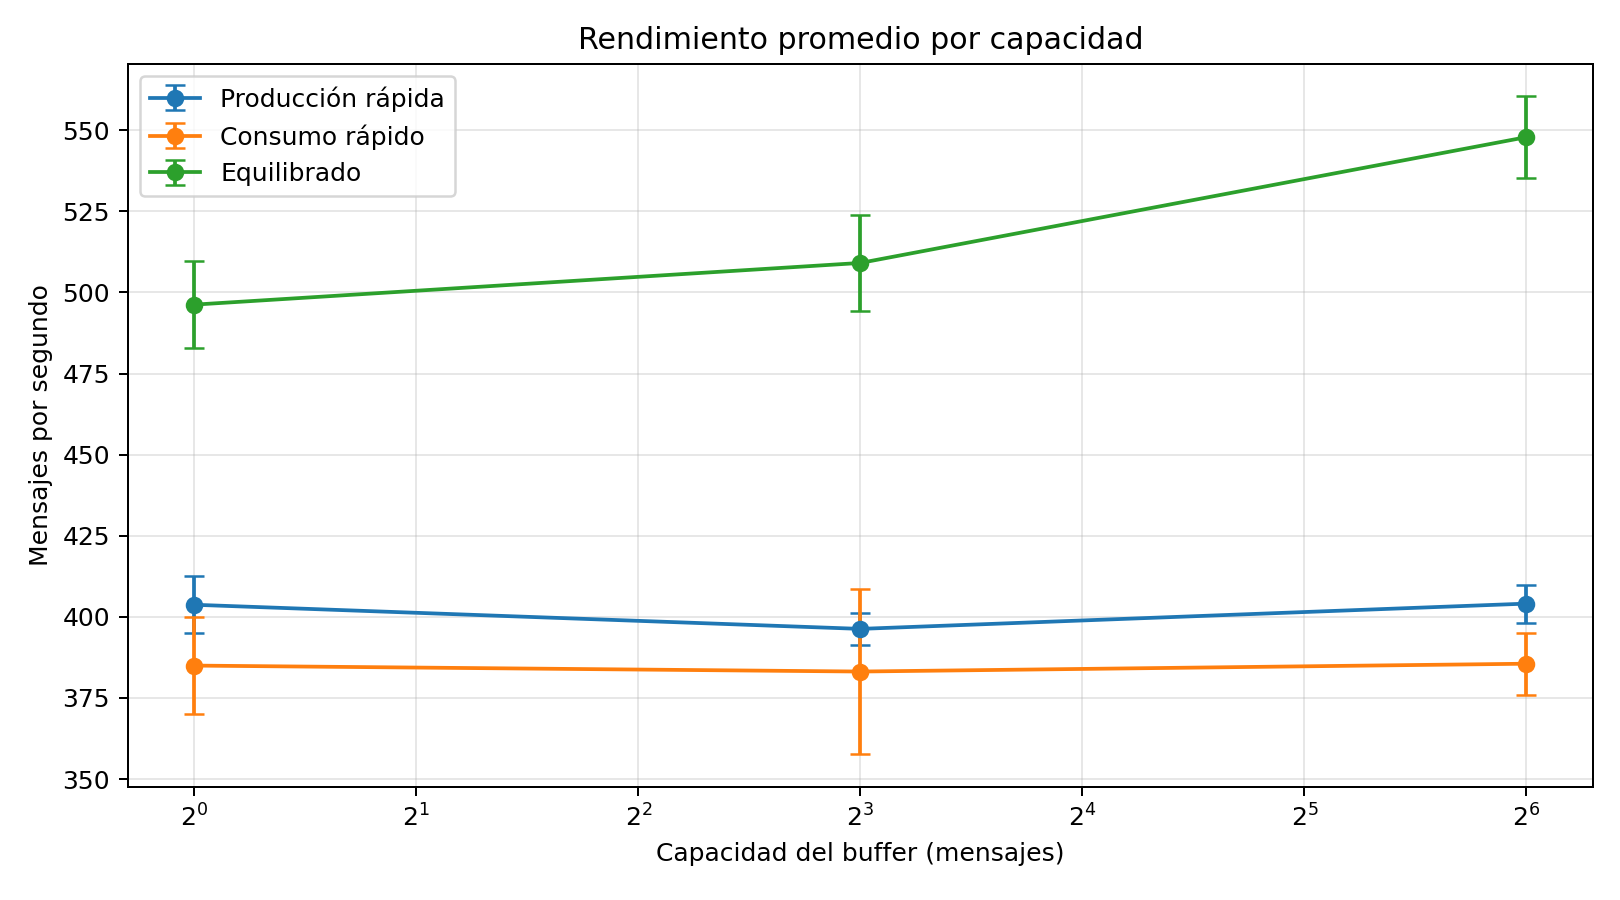
\includegraphics[width=\columnwidth]{rendimiento.png}
\caption{Rendimiento promedio por capacidad y relación entre tasas. Las barras muestran la desviación estándar muestral de cinco corridas.}\label{fig:rendimiento}
\end{figure}

\begin{figure}[htbp]
\centering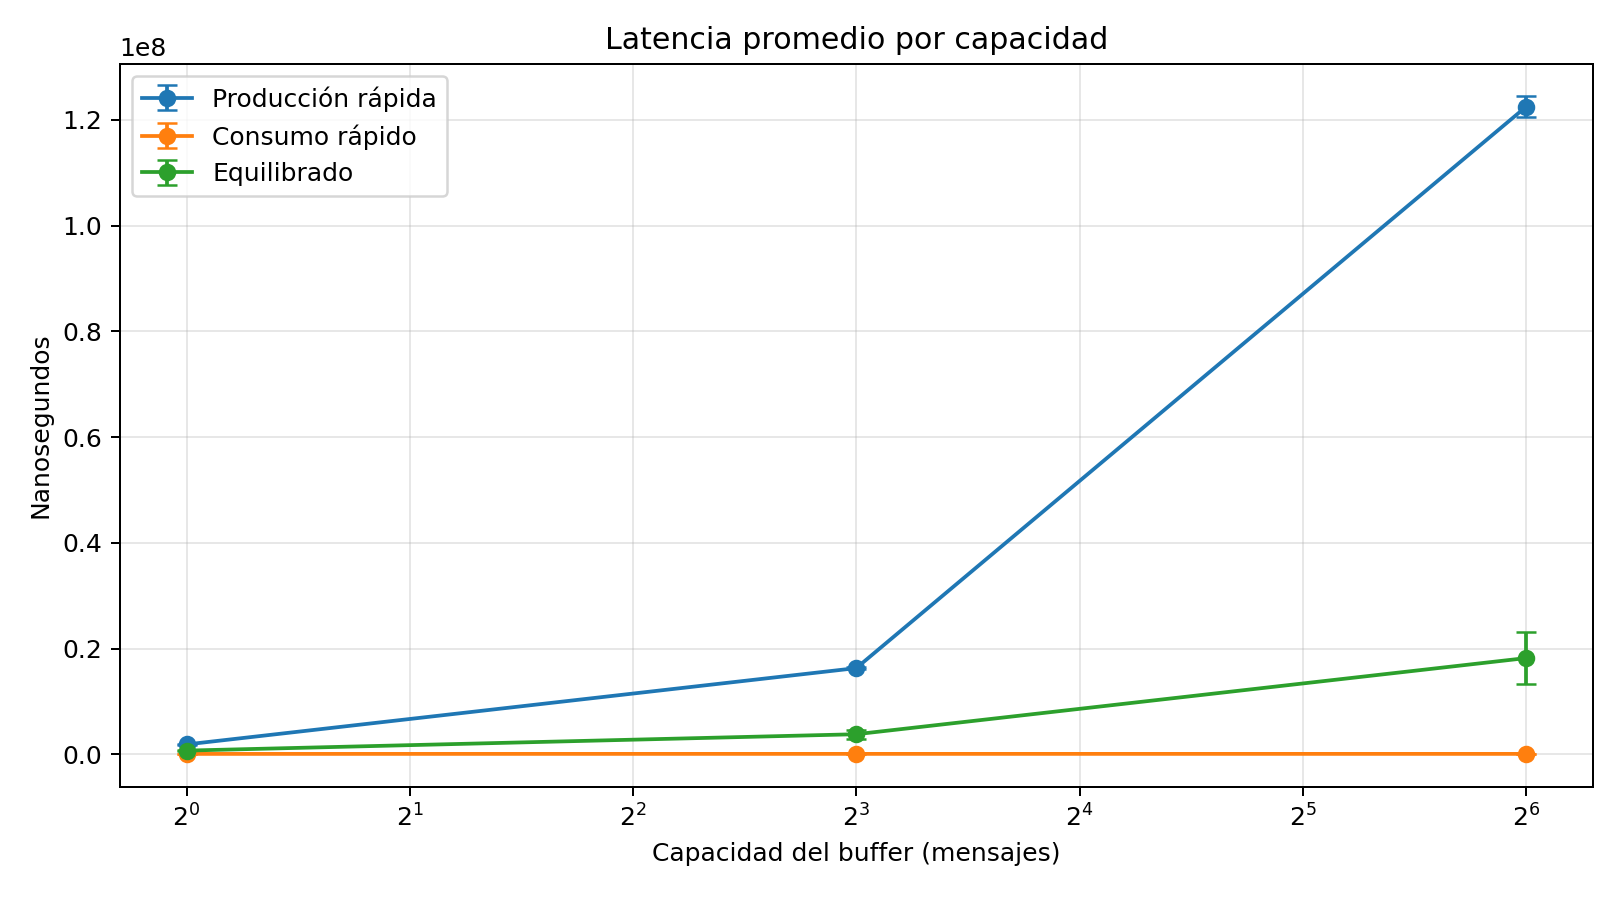
\includegraphics[width=\columnwidth]{latencia_promedio.png}
\caption{Latencia media por capacidad. Valores expresados en milisegundos.}\label{fig:latencia}
\end{figure}

\begin{figure}[htbp]
\centering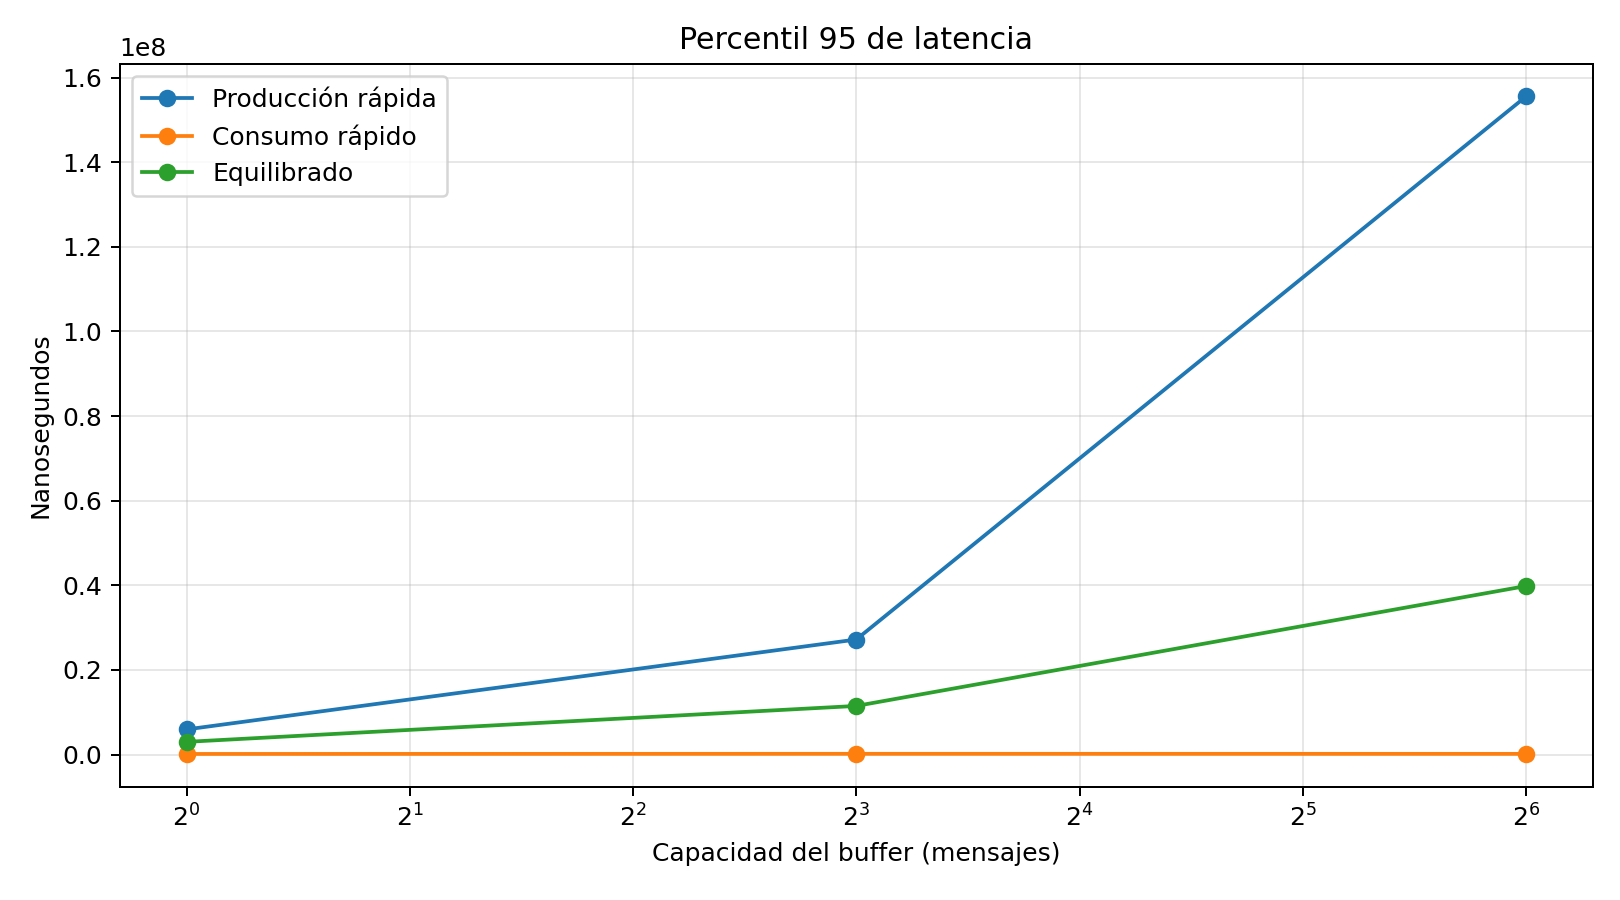
\includegraphics[width=\columnwidth]{latencia_p95.png}
\caption{Promedio del percentil 95 de latencia calculado para cada combinación.}\label{fig:p95}
\end{figure}

\subsection{Interpretación de resultados}
Cuando el consumo fue más rápido que la producción, el rendimiento se mantuvo alrededor de 383--386 mensajes por segundo para las tres capacidades y la latencia media estuvo cerca de 0.11 ms. Esto sugiere que, en este escenario, ampliar el buffer no produjo una mejora relevante en el ritmo de procesamiento observado.

En el escenario equilibrado, el rendimiento medio aumentó de 496.22 a 547.85 mensajes/s entre capacidades 1 y 64; sin embargo, la latencia media también creció de 0.732 a 18.228 ms. Una mayor capacidad permitió acumular más mensajes, pero esa acumulación incrementó el tiempo transcurrido hasta su extracción. El aumento de rendimiento no debe analizarse aisladamente del costo en espera.

Con producción más rápida, el rendimiento permaneció aproximadamente entre 396 y 404 mensajes/s, mientras que la latencia media pasó de 1.900 ms (capacidad 1) a 122.486 ms (capacidad 64). Este es el contraste más marcado: disponer de más espacios no aceleró de manera apreciable al consumidor, pero sí permitió mantener mensajes esperando durante más tiempo. La Figura~\ref{fig:p95} muestra además que ese comportamiento se refleja en las latencias altas.

Los resultados describen este equipo, implementación y conjunto de ejecuciones. No permiten establecer por sí solos significación estadística entre todas las capacidades ni generalizar a otros sistemas. Para reproducir y contrastar estas cifras debe conservarse la identificación exacta de CPU, kernel, compilador y condiciones de carga, y considerar el costo del registro CSV. No se atribuyen diferencias causales a una sola fuente de variación. Aunque los CSV se escriben fuera del mutex, el formateo de los eventos y las operaciones de escritura consumen recursos y pueden modificar el ritmo con el que los trabajadores vuelven a acceder al buffer.

\section{Reproducibilidad y limitaciones}
Los scripts, la matriz de pruebas y los resultados se encuentran en el repositorio del proyecto. Las cifras de la Tabla~\ref{tab:resultados} proceden de \path{results/experimentos/analisis_final/resultados_agrupados.csv}; las gráficas se reconstruyeron a partir de esas mismas cifras y no corresponden a mediciones nuevas. Los parámetros y semillas exactos están en \path{results/experimentos/configuraciones.csv}; los registros detallados de los trabajadores se conservan en la sesión original local \texttt{414cce0564}.

Para repetir una comprobación funcional se dispone de \texttt{make clean}, \texttt{make -j4} y \texttt{make -j4 test}. La validación de entrega debe repetirse sobre una copia limpia del commit elegido. El estrés y los sanitizadores se ejecutaron en Ubuntu 26.04.1 LTS sobre WSL2, kernel 6.18.33.2, GCC 15.2.0 e Intel Core i7-13700H con 20 procesadores lógicos visibles. Estos resultados validan la suite, pero no se usan como referencia de rendimiento ni sustituyen el entorno propio de la sesión experimental.

\textbf{Limitación de trazabilidad experimental:} los consolidados preservados no identifican CPU, memoria, distribución, kernel, GCC ni si la sesión \texttt{414cce0564} se ejecutó directamente o en contenedor. Esos datos no se sustituyen con el entorno posterior de P2-14. La ausencia de ese manifiesto y de las esperas exportadas debe resolverse recuperando la sesión original o repitiendo el experimento antes de la entrega.

\section{Amenazas a la validez}
La validez interna del experimento puede verse afectada por la planificación no determinista de los procesos, la carga de fondo del sistema y el costo de registrar eventos en archivos CSV. Aunque todas las configuraciones siguen el mismo procedimiento y cada combinación se repite cinco veces, no es posible garantizar que las corridas tengan intercalados equivalentes. Las semillas permiten reproducir las pausas locales, pero no controlan las decisiones del planificador del sistema operativo.

Respecto a la validez de construcción, el rendimiento y la latencia representan aspectos distintos del comportamiento. El rendimiento resume la cantidad de mensajes extraídos durante el intervalo operativo, mientras que la latencia mide únicamente el tiempo entre aceptación y extracción. Esta última no incluye el procesamiento privado posterior del consumidor. Por ello, ninguna de las dos medidas debe interpretarse de forma aislada como una caracterización completa del desempeño.

La validez externa está limitada a la implementación, el equipo y las condiciones empleadas. Los resultados no necesariamente se transfieren a otras arquitecturas, versiones del kernel, bibliotecas POSIX o cantidades de procesos. Asimismo, cinco repeticiones permiten describir la variabilidad observada, pero no sustentan por sí solas conclusiones generales ni pruebas de significación estadística. Una evaluación posterior podría incorporar más repeticiones, distintos niveles de concurrencia y mediciones con el registro CSV habilitado y deshabilitado.

\section{Procedencia del material}
El código C, las pruebas, los scripts de análisis y el texto del informe fueron elaborados por el equipo para este proyecto. Las gráficas se generaron con los scripts del repositorio a partir de los CSV publicados. No se incorporó una implementación externa del buffer ni de su coordinación. Dijkstra y Birrell se utilizaron como fundamento conceptual y se citan explícitamente; las APIs POSIX, GCC, GNU Make y Python se emplean como herramientas o interfaces del sistema bajo sus licencias propias, sin redistribuir su código en la entrega. El repositorio académico no concede una licencia general de reutilización sobre el trabajo del equipo.


\section{Conclusiones}
El sistema implementado permite intercambiar mensajes entre procesos independientes mediante una memoria compartida POSIX y un buffer circular FIFO. El uso combinado de mutex y condiciones protege la ocupación, las secuencias globales y el estado operativo; los bloqueos de descriptor añaden una protección necesaria para el cierre y la destrucción cooperativa de recursos.\par
Las pruebas automatizadas y la auditoría de CSV respaldan la conservación, la identidad y el orden de los mensajes en los escenarios ejecutados. La separación entre orden de operación y orden físico de escritura de registros resulta esencial para verificar correctamente un sistema concurrente.\par
El experimento de 45 corridas mostró que el efecto de ampliar el buffer depende de las tasas relativas: con producción rápida la latencia media aumentó de 1.900 a 122.486 ms entre capacidades 1 y 64, mientras el rendimiento se mantuvo cercano a 400 mensajes/s. Por ello, seleccionar la capacidad exige considerar conjuntamente rendimiento, acumulación y tiempo de espera. Las conclusiones se limitan a la implementación, las mediciones y las condiciones evaluadas; no constituyen una garantía general de equidad ni una prueba exhaustiva de todas las carreras.

\begin{thebibliography}{9}
\bibitem{repo} Grupo AEE, ``SOA-P2-GrupoAEE: código, pruebas y resultados experimentales,'' repositorio del proyecto, 2026. \url{https://github.com/lowin22/SOA-P2-GrupoAEE}.
\bibitem{issue16} Grupo AEE, ``P2-16: Informe, README y defensa,'' issue del proyecto, 2026. \url{https://github.com/lowin22/SOA-P2-GrupoAEE/issues/16}.
\bibitem{dijkstra} E. W. Dijkstra, ``Cooperating Sequential Processes,'' EWD123, 1965, secs. 3.2, 3.3, 4.1 y 4.3. \url{https://www.cs.utexas.edu/~EWD/transcriptions/EWD01xx/EWD123.html}.
\bibitem{birrell} A. D. Birrell, ``An Introduction to Programming with Threads,'' SRC Research Report 35, Digital Equipment Corporation, 6 de enero de 1989, secs. ``Using a Mutex: accessing shared data'' y ``Using a Condition variable: scheduling shared resources.'' \url{https://birrell.org/andrew/papers/035-Threads.pdf}.

\end{thebibliography}
\end{document}
